\newpage
\section{数值分析}
\subsection{守恒律方程}
\subsubsection{特征线理论}
我们现在考虑非线性一阶PDE
\begin{equation}
    F(\vecb{D}u,u,\vecb{x})=0,\quad \vecb{x}\in \Omega
    \label{eq:1order}
\end{equation}
以及相应的边界条件
\begin{equation}
    u(\vecb{x})=g(\vecb{x}),\quad \vecb{x}\in \Gamma
    \label{eq:1order_bc}
\end{equation}
其中$\Gamma\subset\partial\Omega,g:\Gamma\to \mathbb{R}$是给定的.\par
设$u$是上述边值问题的解,固定任意点$\vecb{x}\in\Omega$,求一条位于$\Omega$中连接$\vecb{x}$和边界$\Gamma$上某点$\vecb{x}_0$的曲线.根据边界条件可知在$\Gamma$上$u=g$,我们知道$u$在一个端点$\vecb{x}_0$上的值,我们希望可以求出$u$在这条曲线上的值,那么$u(\vecb{x})$就求出来了.\par
设这条曲线为$\vecb{x}(s)=(x_1(s),x_2(s),\cdots,x_n(s)),s\in I\subset\mathbb{R}$.假设$u$是\eqref{eq:1order}的$C^2$解,再定义$z(s)=u(\vecb{x}(s))$,另外再设
$$
\vecb{p}(s)=\vecb{D}_{\vecb{x}}u(\vecb{x}(s))=(p_1(s),p_2(s),\cdots,p_n(s))
$$
其中$p_i(s)=\frac{\partial u}{\partial x_i}(\vecb{x}(s))$.根据一系列不怎么复杂的计算,我们得到下面的ODE方程组
\begin{equation}
    \begin{cases}
    \dot{\vecb{p}}(s) &= -\vecb{D}_{\vecb{x}}F(\vecb{p}(s),z(s),\vecb{x}(s))-F_{z}(\vecb{p}(s),z(s),\vecb{x}(s))\vecb{p}(s)\\ 
    \dot{z}(s) &= \vecb{D}_{\vecb{p}}F(\vecb{p}(s),z(s),\vecb{x}(s))\cdot\vecb{p}(s)\\
    \dot{\vecb{x}}(s) &= \vecb{D}_{\vecb{p}}F(\vecb{p}(s),z(s),\vecb{x}(s))
\end{cases}
\label{eq:char_ode}
\end{equation}
$$
F(\vecb{p}(s),z(s),\vecb{x}(s))\equiv 0
$$
我们将\eqref{eq:char_ode}这$2n+1$个一阶常微分方程构成的方程组叫做非线性一阶PDE\eqref{eq:1order}的特征线方程组,曲线$\vecb{x}(s)$叫做投影特征.\par
如果我们给定下面的线性齐次方程
$$
F(\vecb{D}u,u,\vecb{x})=\vecb{b}(\vecb{x})\cdot\vecb{D}u+c(\vecb{x})u=0
$$
那么$F(\vecb{p},z,\vecb{x})=\vecb{b}(\vecb{x})\cdot\vecb{p}+c(\vecb{x})z$.因此特征线方程组\eqref{eq:char_ode}可以写成
$$
\begin{cases}
    \dot{\vecb{x}}(s)&=\vecb{b}(\vecb{x}(s))\\
    \dot{z}(s)&=-c(\vecb{x}(s))z(s)
\end{cases}
$$
\qquad 下面考虑拟线性方程
$$
F(\vecb{D}u,u,\vecb{x})=\vecb{b}(u(\vecb{x}),\vecb{x})\cdot\vecb{D}u(\vecb{x})+c(u(\vecb{x}),\vecb{x})u=0
$$
此时$F(\vecb{p},z,\vecb{x})=\vecb{b}(z,\vecb{x})\cdot\vecb{p}+c(z,\vecb{x})z$.因此特征线方程组\eqref{eq:char_ode}可以写成
$$
\begin{cases}
    \dot{\vecb{x}}(s)&=\vecb{b}(z(s),\vecb{x}(s))\\
    \dot{z}(s)&=-c(z(s),\vecb{x}(s))z(s)
\end{cases}
$$
\qquad 考虑标量守恒律:在$\Omega=\mathbb{R}^n\times (0,\infty)$上
$$
G(\vecb{D}u,u_t,u,\vecb{x},t)=u_t+\operatorname{div}\vecb{F}(u)=u_t+\vecb{F}'(u)\cdot\vecb{D}u=0
$$
初始条件为
$$
u(\vecb{x},0)=g(\vecb{x}),\quad \vecb{x}\in\mathbb{R}^n
$$
我们记$t=x_{n+1},\vecb{q}=(\vecb{p},p_{n+1}),\vecb{y}=(\vecb{x},t)$.其中$p_{n+1}=u_t$.因此方程转化为
$$
G(\vecb{q},z,\vecb{y})=p_{n+1}+\vecb{F}'(z)\cdot\vecb{p}=(\vecb{F}'(z),1)\cdot\vecb{q}=0
$$
经过简单的计算可以得出
$$
\vecb{D}_{\vecb{q}}G=(\vecb{F}'(z),1),\quad \vecb{D}_{\vecb{y}}G=0,\quad \vecb{D}_{z}G=\vecb{F}''(z)\cdot\vecb{p}
$$
所以特征方程组为
$$
\begin{cases}
    \dot{\vecb{q}}(s)&=-(\vecb{F}''(z(s))\cdot\vecb{p}(s))\vecb{q}(s)\\
    \dot{z}(s)&=0\\
    \dot{\vecb{y}}(s)&=(\vecb{F}'(z(s)),1)
\end{cases}
$$
关于最后一个等式我们可以看到
$$
\frac{\mathrm{d}x}{\mathrm{d}s}=\vecb{F}'(z(s)),\quad \frac{\mathrm{d}t}{\mathrm{d}s}=1
$$
因此我们不妨直接设参数$s=t$.由此得到第二个等式的意义:解$u$在特征线上是常数.并且由$\frac{\mathrm{d}x}{\mathrm{d}t}=\vecb{F}'(z(t))$知道投影特征线在空间中的演化速度为$\vecb{F}'(z(t))$.\par
由于$\frac{\mathrm{d}z}{\mathrm{d}t}=0$,所以
$$
z(t)=z(0)=u(\vecb{x}(0),0)=g(\vecb{x})
$$
带入到轨迹方程中得到$\frac{\mathrm{d}x}{\mathrm{d}t}=\vecb{F}'(g(\vecb{x}))$,这就说明我们固定一点$\vecb{x}_0\in\mathbb{R}^n$,特征线的斜率恒定为$\vecb{F}'(g(\vecb{x}_0))$.因此特征线是时空平面中的直线.由此对从$\vecb{x}_0$出发的轨迹方程积分可以得到特征方程
$$
\vecb{x}(t)=\vecb{x}_0+\vecb{F}'(g(\vecb{x}_0))t
$$
从上面的形式我们也可以观察到,初值是可以影响到特征线的斜率的.\par
\subsubsection{一维标量守恒律}
我们看一个例子:Burgers方程的初值问题
$$
\begin{cases}
\begin{alignedat}{2}
    u_t + \left( \frac{u^2}{2} \right)_x &= 0,   \quad && (x, t) \in \mathbb{R} \times (0, \infty) \\
    u(x, 0)                             &= g(x), \quad && x \in \mathbb{R}
\end{alignedat}
\end{cases}
$$
我们取初值数据为
$$
g(x)=
\begin{cases}
    1,& \text{若}x\leqslant 0\\
    1-x,& \text{若}x\in [0,1]\\
    0,& \text{若}x\geqslant 1
\end{cases}
$$
按照特征线方程的样子,我们很容易求出特征线的方程为
$$
x(t)=
\begin{cases}
    x_0+t,& \text{若}x_0\leqslant 0\\
    x_0+(1-x_0)t,& \text{若}x_0\in [0,1]\\
    x_0,& \text{若}x_0\geqslant 1
\end{cases}
$$
我们很容易就可以将图像画出来,不过需要注意的是,我们将$x$作为横轴.$x_0$就是从$x$轴上出发的点.
\begin{center}
    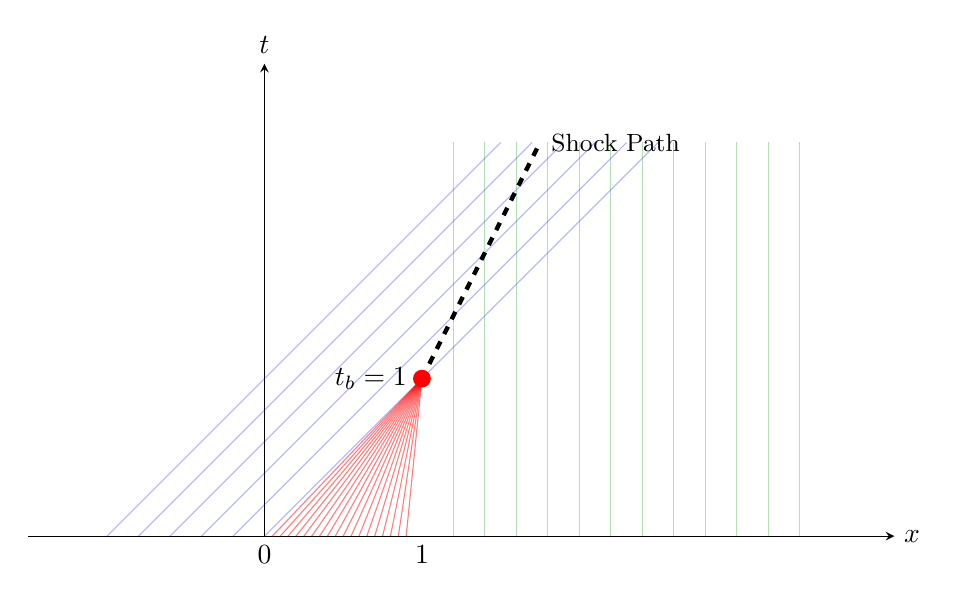
\begin{tikzpicture}[>=stealth, scale=2]
    % 坐标轴
    \draw[->] (-1.5,0) -- (4,0) node[right] {$x$};
    \draw[->] (0,0) -- (0,3) node[above] {$t$};
    
    % 辅助刻度
    \node[below] at (0,0) {$0$};
    \node[below] at (1,0) {$1$};

    % 1. 左侧蓝色特征线 (间距 0.2)
    \foreach \xzero in {-1, -0.8, ..., 0} {
        \draw[blue, opacity=0.3] (\xzero, 0) -- (\xzero + 2.5, 2.5);
    }
    
    % 2. 中间红色特征线 (间距更小: 0.05)
    \foreach \xzero in {0.05, 0.1, ..., 0.95} {
        % 它们在 t=1 时相交于 x=1
        \draw[red, opacity=0.5] (\xzero, 0) -- (1, 1);
    }
    
    % 3. 右侧绿色特征线 (间距 0.2)
    \foreach \xzero in {1.2, 1.4, ..., 3.5} {
        \draw[green!60!black, opacity=0.3] (\xzero, 0) -- (\xzero, 2.5);
    }

    % 4. 激波形成后的轨迹 (t > 1)
    % 激波方程: x_s(t) = 1 + 0.5*(t-1)
    \draw[black, ultra thick, dashed] (1,1) -- (1.75, 2.5) 
        node[right, font=\small] {Shock Path};

    % 强调 Breaking Point
    \filldraw[red] (1,1) circle (1.5pt) node[left, black, xshift=-2pt] {$t_b=1$};

\end{tikzpicture}
\end{center}
从图上我们看到了特征线相交.\par
如果我们考虑下面的初值问题
$$
\left\{  \begin{array}{ll} {\partial }_{t}u + {\partial }_{x}\left( \frac{{u}^{2}}{2}\right)  = 0 & \text{ for }x \in  \left\lbrack  {0,{2\pi }}\right\rbrack  ,t > 0, \\  u\left( {x,0}\right)  = \sin x & \text{ for }x \in  \left\lbrack  {0,{2\pi }}\right\rbrack  . \end{array}\right.
$$
\qquad 容易求出特征线为
$$
x(t)=x(0)+\sin(x(0))t
$$
并且$u$沿此特征线为常数$g(x(0))=\sin(x(0))$.对于固定的$(x,t)$,因为$x(0)=x-t\sin(x(0))$,于是$u$满足下面的方程
$$
u-\sin(x-tu)=0
$$
这是一个关于$u$的非线性方程.在此之前我们先关注$u-\sin(x-tu)=0$,由隐函数定理可知
$$
\frac{\partial u}{\partial x} = \frac{\cos(x-tu)}{1+t\cos(x-tu)},\quad \frac{\partial u}{\partial t} = -\frac{u\cos(x-tu)}{1+t\cos(x-tu)}
$$
当分母$1+t\cos(x-tu)=0$时,导数$\frac{\partial u}{\partial x}$无界,此时$u$产生间断,我们现在寻找第一次发生间断的时间$t_b$,显然
$$
t_b=\min\left(-\frac{1}{\cos(x-tu)}\right)=1
$$
当$t=1$时,$\cos(x-tu)=-1$,解得$x-u=(2k+1)\pi$,根据方程$u-\sin(x-u)=0$以及$x\in [0,2\pi]$得到$x=\pi$,这说明$t=1$时在$x=\pi$处产生间断,激波形成.\par
事实上,通过特征线的表达式我们可以看出,当$x\in [0,\pi)$时,特征线的斜率$\sin(x(0))$为正,因此特征线向右传播;当$x\in (\pi,2\pi]$时,特征线的斜率$\sin(x(0))$为负,因此特征线向左传播;当$x=\pi$时,特征线的斜率$\sin(x(0))$为零,因此特征线垂直于时间轴.并且根据$\sin x$关于$x=\pi$中心对称,那么在$x-t$平面上特征线关于$x=\pi$对称地相交于射线$x=\pi$上.\par
\begin{center}
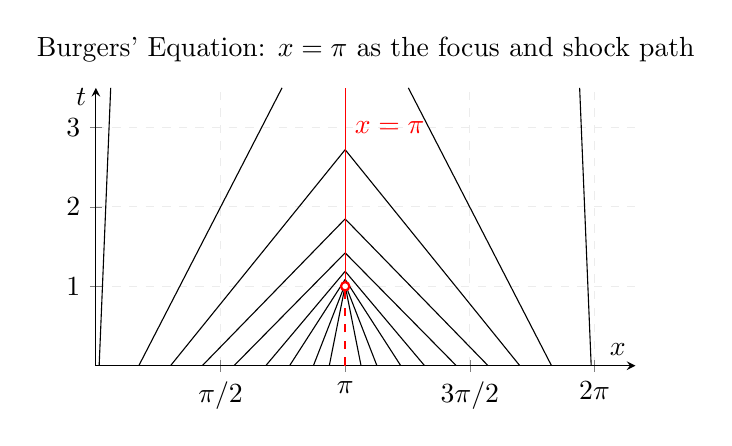
\begin{tikzpicture}
    \begin{axis}[
        axis lines = middle,
        xmin = 0, xmax = 6.8, 
        ymin = 0, ymax = 3.5, 
        xlabel = {$x$},
        ylabel = {$t$},
        ylabel style={
        at={(axis description cs:0,0.9)}, % 定位到左上角 (0,1)
        anchor=south east,              % 确保标签在轴的左上方
    },
        xtick = {0, 1.5708, 3.14159, 4.71239, 6.28318},
        xticklabels = {0, $\pi/2$, $\pi$, $3\pi/2$, $2\pi$},
        ytick = {0, 1, 2, 3},
        unit vector ratio*=1 1, 
        grid = major,
        grid style = {dashed, gray!15},
        title = {Burgers' Equation: $x=\pi$ as the focus and shock path}
    ]

        \def\xpi{3.14159265}
        \def\tshock{1.0}

        % --- 1. 绘制特征线 ---
        \foreach \delta in {0.2, 0.4, 0.7, 1.0, 1.4, 1.8, 2.2, 2.6, 3.1} {
            
            % 处理左侧 (pi - delta) 和 右侧 (pi + delta)
            \foreach \direction in {-1, 1} {
                \pgfmathsetmacro{\xzero}{\xpi + \direction * \delta}
                \pgfmathsetmacro{\u}{sin(\xzero r)}
                
                % 计算撞击时间
                \ifdim \delta pt < 0.01pt
                    \def\tend{3.5}
                \else
                    \pgfmathsetmacro{\tcalc}{(\xpi - \xzero) / \u}
                    \ifdim \tcalc pt > 1.0pt
                        \pgfmathsetmacro{\tend}{min(3.5, \tcalc)}
                    \else
                        \def\tend{3.5}
                    \fi
                \fi

                \addplot[domain=0:\tend, samples=2, thin] 
                ({\xzero + x*sin(\xzero r)}, {x});
            }
        }

        % --- 2. 绘制从 x 轴出发的参考线/激波线 ---
        
        % t=0 到 t=1: 虚线（特征线汇聚线）
        \draw[thick, red, dashed] (axis cs: \xpi, 0) -- (axis cs: \xpi, 1);
        
        % t=1 到 ymax: 实线（激波轨迹）
        \draw[thin, red] (axis cs: \xpi, 1) -- (axis cs: \xpi, 3.5)
            node[right, pos=0.8] {$x=\pi$};

        % 标注激波起始点
        \draw[fill=white, draw=red, thick] (axis cs: \xpi, 1) circle (1.5pt);

    \end{axis}
\end{tikzpicture}
\end{center}
记$f(u)=u-\sin(x-tu)$.给定$(x,t)$求$u$的值,此时就等价于求解$f(u)=0$.因此我们可以在$t\in [0,1)$的时间区间内求解上述非线性方程.\par
利用Newton迭代法,首先我们需要求出$f'(u)$,有$f'(u)=1+t\cos(x-tu)$,于是现在得到迭代公式
$$
u_{n+1}=u_n-\frac{f(u_n)}{f'(u_n)}=u_n-\frac{u_n-\sin(x-tu_n)}{1+t\cos(x-tu_n)}
$$
值得注意的是,因为我们要求$t\in[0,1)$,那么$f'(u)$不会为零,这保证了迭代是合理的.\par
利用下面的算法
\begin{algorithm}[H]
\caption{牛顿法求解隐式解 $u = \sin(x - tu)$}
\begin{algorithmic}[1]
\State \textbf{Input:} 空间位置 $x$,时间 $t$,初始猜测值 $u^{(0)}$,容差 $\varepsilon$,最大迭代次数 $M$
\State \textbf{Initialization:} $k = 0$,误差 err $= \infty$
\While {err $> \varepsilon$ \textbf{and} $k < M$}
    \State $f(u^{(k)}) = u^{(k)} - \sin(x - t \cdot u^{(k)})$
    \State $f'(u^{(k)}) = 1 + t \cdot \cos(x - t \cdot u^{(k)})$
    \State 更新解:
    $$u^{(k+1)} = u^{(k)} - \frac{f(u^{(k)})}{f'(u^{(k)})}$$
    \State err $= |u^{(k+1)} - u^{(k)}|$
    \State $k = k + 1$
\EndWhile
\State \textbf{Output:} $u^{(k)}$
\end{algorithmic}
\end{algorithm}
下面我们将$[0,2\pi]$等分为500份,并按步长50取值作为空间位置$x$.下面左侧的表格给出了$t=0,0.5,0.9$时刻$u$在不同位置的数值解,右侧的表格给出了对应时间的函数图像.\par
  \begin{figure}[H]
    \vspace{0pt}
    \centering
    % --- 左侧：数值表格 ---
    \begin{minipage}[t]{0.45\textwidth}
      
        \centering
        \captionof{table}{各空间点 $x$ 在不同时刻 $t$ 的数值解}
        \label{tab:evolution}
        \renewcommand{\arraystretch}{1.25} % 配合宽页边距，稍微拉开行高
        \small
        \begin{tabular}[t]{|c|c|c|c|}
        \hline
        \textbf{$x$} & \textbf{$u(x, 0.0)$} & \textbf{$u(x, 0.5)$} & \textbf{$u(x, 0.9)$} \\ \hline
        0.0000 & 0.0000 & 0.0000 & 0.0000 \\ \hline
        0.6283 & 0.5878 & 0.4105 & 0.3275 \\ \hline
        1.2566 & 0.9511 & 0.7665 & 0.6337 \\ \hline
        1.8850 & 0.9511 & 0.9842 & 0.8856 \\ \hline
        2.5133 & 0.5878 & 0.8752 & 0.9991 \\ \hline
        3.1416 & 0.0000 & 0.0000 & 0.0000 \\ \hline
        3.7699 & -0.5878 & -0.8752 & -0.9991 \\ \hline
        4.3982 & -0.9511 & -0.9842 & -0.8856 \\ \hline
        5.0265 & -0.9511 & -0.7665 & -0.6337 \\ \hline
        5.6549 & -0.5878 & -0.4105 & -0.3275 \\ \hline
        6.2832 & 0.0000 & -0.0000 & -0.0000 \\ \hline
        \end{tabular}
    \end{minipage}
    \hfill
    % --- 右侧：三图堆叠 ---
    \begin{minipage}[t]{0.5\textwidth}
      \vspace{0pt}
        \centering
        \caption{对应时刻的数值解曲线演化图}
        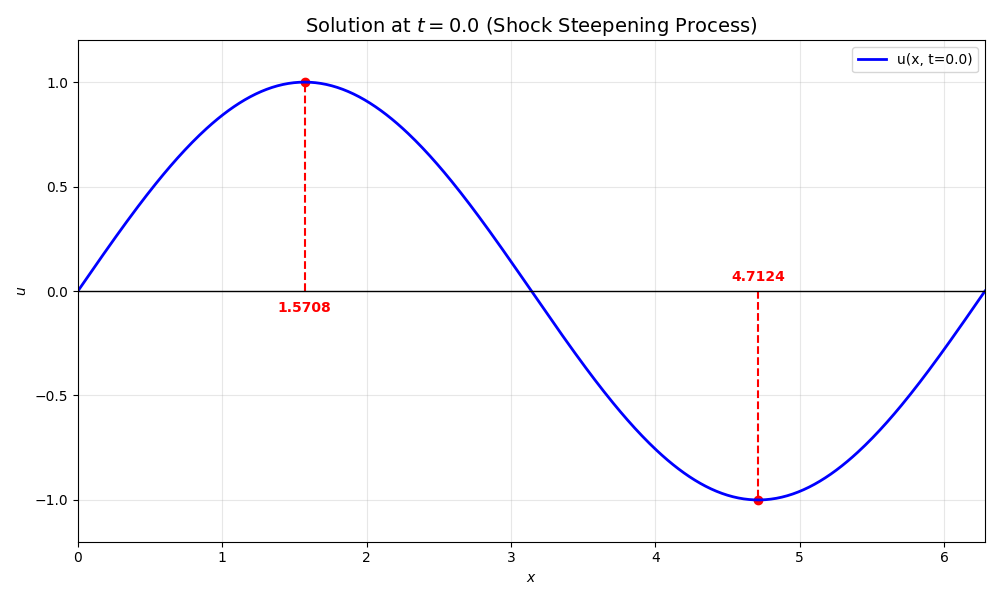
\includegraphics[width=0.6\linewidth]{Figure/t0.png}
        \\[0.1cm] % 紧凑排版
        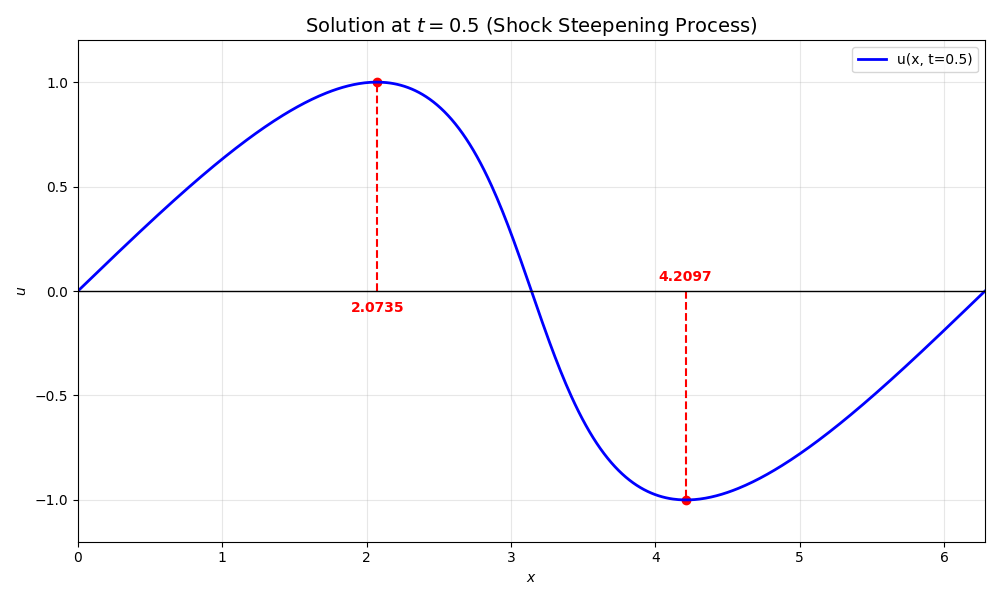
\includegraphics[width=0.6\linewidth]{Figure/t1.png}
        \\[0.1cm]
        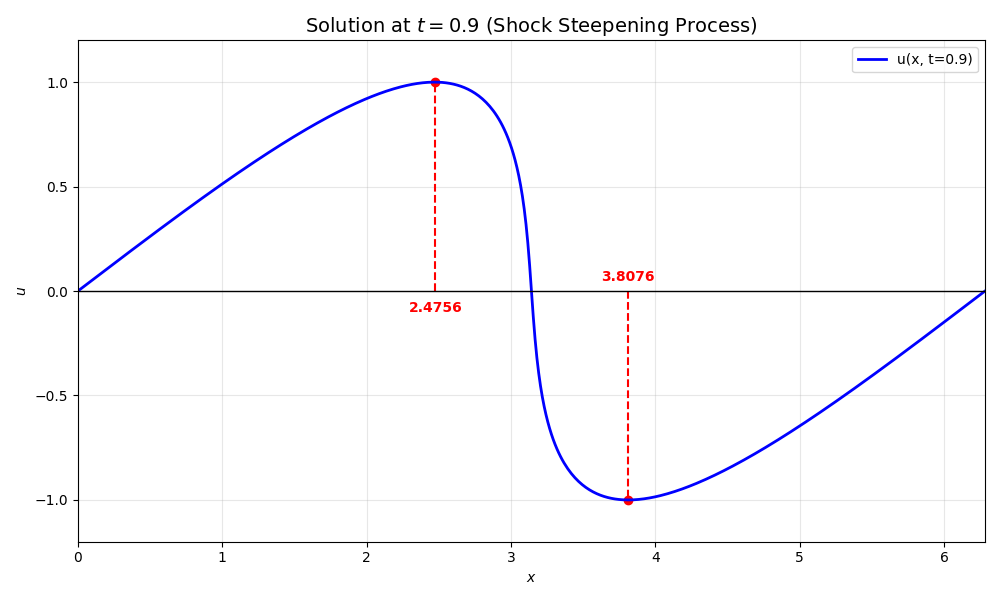
\includegraphics[width=0.6\linewidth]{Figure/t2.png}
        
        \label{fig:plots_group}
    \end{minipage}
\end{figure}
图像中两条虚线是函数最高点与最低点对应到$x$轴的坐标,从上面的表格与图可以看出,随着时间$t$的增加,$x=\pi$左侧的函数图像如同波浪一样往右传播,$x=\pi$右侧的函数往左传播,最终形成间断.从我们的直觉来看,随着时间的演化,函数图像会变成Z字型,然而这不符合数学事实.其实到后面我们将看到,函数图像只会在$x=\pi$垂直坠落.\par
\subsubsection{Rankine-Hugoniot条件}
现在我们考虑一维标量守恒律的初值问题
\begin{equation}
    \begin{cases}
        \begin{alignedat}{2}
             u_t + F(u)_x &= 0, && (x,t)\in\mathbb{R}\times (0,\infty)\\
             u(x, 0) &= g(x), \quad && x \in \mathbb{R}
        \end{alignedat}
\label{eq:1dcl}
\end{cases}
\end{equation}
其中$F:\mathbb{R}\to\mathbb{R}, g:\mathbb{R}\to\mathbb{R}$是给定的函数.\par
从上面的分析中我们可以看出,\eqref{eq:1dcl}一般没有在$t>0$上的连续解.因此我们现在寻找一种弱解.\par
设$v:\mathbb{R}\times [0,\infty)\to\mathbb{R}$是光滑且具有紧支集的函数.那么
$$
\begin{aligned}
    0 &= \int_0^\infty\int_{-\infty}^\infty (u_t+F(u)_x)v\mathrm{d}x\mathrm{d}t\\
    &= \int_0^\infty\int_{-\infty}^\infty u v_t\mathrm{d}x\mathrm{d}t -\int_{-\infty}^\infty uv\mathrm{d}x|_{t=0}-\int_0^\infty\int_{-\infty}^\infty F(u)v_x\mathrm{d}x\mathrm{d}t\\
\end{aligned}
$$
再根据边界条件$u(x,0)=g(x)$得到下面的恒等式
$$
\int_0^\infty\int_{-\infty}^\infty (u v_t+F(u)v_x)\mathrm{d}x\mathrm{d}t + \int_{-\infty}^\infty g(x)v(x,0)\mathrm{d}x = 0
$$
\qquad 如果上式对每一个检验函数$v$都成立,则称$u\in L^{\infty}(\mathbb{R}\times (0,\infty))$是\eqref{eq:1dcl}的弱解.\par
\begin{center}
\tikzset{every picture/.style={line width=0.5pt}} 
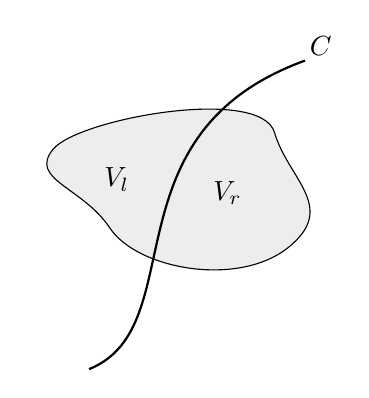
\begin{tikzpicture}[x=0.5pt,y=0.5pt,yscale=-1,xscale=1]

% --- 1. 整体填充 V_l 和 V_r 所在的区域 ---
% 使用你原本的 Bezier 坐标，设置为填充 gray!20，同时保留描边
\draw [fill={rgb, 255:red, 220; green, 220; blue, 220}, fill opacity=0.5]  
    (239,93) .. controls (257,71) and (389,47) .. (399,81) .. 
    controls (409,115) and (445,135) .. (409,164) .. 
    controls (373,193) and (300,180) .. (280,150) .. 
    controls (260,120) and (221,115) .. (239,93) -- cycle;

% --- 2. 画中间的曲线 C ---
% 增加 thick 使其在灰色背景中更清晰，并在末端标注 C
\draw [thick] (265,252) .. controls (341,221) and (275,82) .. (421,29) 
    node [anchor=south west, xshift=-2pt, yshift=-2pt] {$C$};

% --- 3. 放置文字标注 ---
% 调整 V_l 和 V_r 的位置，确保它们在灰色区域内清晰可见
\draw (285,115) node [font=\normalsize] {$V_l$};
\draw (365,125) node [font=\normalsize] {$V_r$};

\end{tikzpicture}
\end{center}
\qquad 我们知道,特征线的交叉形成了间断点.下面我们获得间断点的传播速率.假设在某一开区域$V\subset \mathbb{R}\times (0,\infty)$内,$u$在光滑曲线$C$的每一侧是光滑的.现在假设$u$是\eqref{eq:1dcl}的弱解,且$u$及其一阶导数在$V_l,V_r$内是一致连续的.选择一个紧支集包含在$V_l$内的检验函数$v$,那么
$$
0=\int_0^\infty\int_{-\infty}^\infty (u v_t+F(u)v_x)\mathrm{d}x\mathrm{d}t=-\int_0^\infty\int_{-\infty}^\infty (u_t+F(u)_x)v\mathrm{d}x\mathrm{d}t
$$
上式对所有紧支集包含在$V_l$内的检验函数$v$都成立.因此$u_t+F(u)_x=0,(x,t)\in V_l$.同理,$u_t+F(u)_x=0,(x,t)\in V_r$.\par
现在再选择一个检验函数$v$,使得$v$的支集包含在$V$内,并且$v$在$C$上不必为零.因此
$$
\begin{aligned}
    0 &=\int_0^\infty\int_{-\infty}^\infty (u v_t+F(u)v_x)\mathrm{d}x\mathrm{d}t\\
    &=\iint_{V_l} (u v_t+F(u)v_x)\mathrm{d}x\mathrm{d}t+\iint_{V_r} (u v_t+F(u)v_x)\mathrm{d}x\mathrm{d}t\\
    &=\left\{-\iint_{V_l} (u_t+F(u)_x)v\mathrm{d}x\mathrm{d}t - \iint_{V_r} (u_t+F(u)_x)v\mathrm{d}x\mathrm{d}t\right\}\\
    &+\left\{\int_{C}[u_l\nu_2+F(u_l)\nu_1]v\mathrm{d}l-\int_{C}[u_r\nu_2+F(u_r)\nu_1]v\mathrm{d}l\right\}\\
    &= \int_{C} \left[(u_l-u_r)\nu_2+(F(u_l)-F(u_r))\nu_1\right]v\mathrm{d}l
\end{aligned}
$$
其中$(\nu_1,\nu_2)$是曲线$C$的单位法向量,从$V_l$指向$V_r$.$u_l,u_r$分别表示在曲线$C$左侧和右侧的极限值.因为上式对每一个检验函数$v$都成立,所以沿着曲线$C$有
$$
(u_l-u_r)\nu_2+(F(u_l)-F(u_r))\nu_1=0
$$
\qquad 假设曲线$C=\{(x,t):x=s(t),s:[0,\infty)\to\mathbb{R}\text{是一个光滑函数}\}$,则我们现在取$(\nu_1,\nu_2)=(\frac{-\dot{s}}{\sqrt{1+(\dot{s})^2}}, \frac{1}{\sqrt{1+(\dot{s})^2}})$,那么在$V$中沿着$u$的间断曲线$C$有
$$
F(u_l)-F(u_r)=\dot{s}(u_l-u_r)
$$
如果我们记$[u]=u_l-u_r$和$[F(u)]=F(u_l)-F(u_r)$,那么上式可以写成
$$
[F(u)]=\dot{s}[u]
$$
因此间断点的传播速率$\dot{s}$满足上式.我们称上式为\textbf{Rankine-Hugoniot条件}.\par
回顾初值问题
$$
\left\{  \begin{array}{ll} {\partial }_{t}u + {\partial }_{x}\left( \frac{{u}^{2}}{2}\right)  = 0 & \text{ for }x \in  \left\lbrack  {0,{2\pi }}\right\rbrack  ,t > 0, \\  u\left( {x,0}\right)  = \sin x & \text{ for }x \in  \left\lbrack  {0,{2\pi }}\right\rbrack  . \end{array}\right.
$$
那么根据Rankine-Hugoniot条件,激波的传播速率为
$$
\dot{s}=\frac{F(u_l)-F(u_r)}{u_l-u_r}=\frac{\frac{u_l^2}{2}-\frac{u_r^2}{2}}{u_l-u_r}=\frac{u_l+u_r}{2}
$$
因为$\sin x$关于$x=\pi$中心对称,所以$u_l=-u_r$,因此$\dot{s}=0$.这说明激波在$x=\pi$处形成后,一直停留在$x=\pi$处不动.\par
\subsubsection{熵条件}
如果我们给定初始条件
$$
g(x)=
\begin{cases}
    0,& \text{if}\; x<0\\
    1,& \text{if}\; x>0
\end{cases}
$$
那么很容易求出特征线方程为
$$
x(t)=
\begin{cases}
    x(0),& \text{if}\; x<0\\
    x(0)+t,& \text{if}\; x>0
\end{cases}
$$
根据Rankine-Hugoniot条件,激波传播速率为$\dot{s}=\frac{1}{2}$,因此激波线为$x=\frac{1}{2}t$.\par
为了直观,我们画出特征线示意图如下
\begin{center}
    \begin{tikzpicture}[>=stealth, scale=1.5]

    % 坐标轴
    \draw[->] (-2.5,0) -- (4,0) node[right] {$x$};
    \draw[->] (0,0) -- (0,3) node[above] {$t$};
    \node at (0,0) [below left] {$O$};

    % 1. 左侧特征线 (x < 0) - 垂直向上 (速度为0)
    \foreach \x in {-2.0, -1.5, -1.0, -0.5} {
        \draw[->,blue, thick] (\x, 0) -- (\x, 2.5);
    }
    \node[blue] at (-1.25, 2.7) {\small $x(t) = x(0)$};

    % 2. 右侧特征线 (x > 0) - 斜向右上方 (速度为1)
    \foreach \x in {0.5, 1.0, 1.5, 2.0} {
        \draw[->,red, thick] (\x, 0) -- (\x+2.5, 2.5);
    }
    \node[red] at (3, 2.7) {\small $x(t) = x(0) + t$};

    % 3. 特征真空区 (The Vacuum Region)
    \fill[gray, opacity=0.1] (0,0) -- (0,2.5) -- (2.5,2.5) -- cycle;
    \node[text width=3cm, align=center] at (0.8, 1.8) {\footnotesize \textbf{特征真空区}};

    % 4. 非物理激波 (Expansion Shock) - 取 s=0.5
    \draw[dashed, line width=1.5pt, black] (0,0) -- (2.5,2.5) ;
\end{tikzpicture}
\end{center}
我们发现在特征真空区$\{0<x<t\}$,特征线方法并不能为我们提供任何关于解的信息.如果取
$$
u_1(x,t)=
\begin{cases}
    0,&\text{if}\; x<\frac{t}{2}\\[4pt]
    1,&\text{if}\; x<\frac{t}{2}\\
\end{cases}
$$
那么$u_1$是初值问题的一个弱解,但你会发现它的一部分信息并不从初值演化而来,而是从间断点无中生有得到的.\par
再构造另一种解
$$
u_2(x,t)=
\begin{cases}
    0,&\text{if}\; x<0\\
    \frac{x}{t},&\text{if}\; 0<x<t\\
    1,&\text{if}\; x>t
\end{cases}
$$
这也是上述初值问题的一个弱解,不过它将特征真空区域利用从原点出发的射线填满了,这符合物理逻辑.\par
某些情况下,弱解并不唯一,并且其中有些解是不具有物理意义的.因此,我们需要一个能够判断某解是否可接受的标准,并且还需要验明该标准足以取得一个具备相关物理意义的唯一解.我们将这种唯一解称为熵解.\par
判断满足$u_l<u_r$的间断解是否是物理解的熵条件---\textbf{Lax熵条件}
$$
\forall u\in (u_l,u_r):\frac{F(u)-F(u_l)}{u-u_l}\geqslant \dot{s}\geqslant \frac{F(u)-F(u_r)}{u-u_r}
$$
\qquad 为了进一步简化,假设$F(u)$是严格凸函数,那么间断点处的激波速率为
$$
\begin{aligned}
    \dot{s}\leqslant \frac{F(u)-F(u_l)}{u-u_l} &=\frac{F(u_l)+F'(u_l)(u-u_l)+\frac{1}{2}F''(\xi)(u-u_l)^2-F(u_l)}{u-u_l}\\
                                               &= F'(u_l)+\frac{1}{2}F''(\xi)(u-u_l)
\end{aligned}
$$
\qquad 如果$u_l>u_r$,那么对于任意$u\in (u_r,u_l)$有$u-u_l<0$,又因为$F''>0$,因此$\dot{s}<F'(u_l)$,同理有$\dot{s}>F'(u_r)$.这就产生了简化版的Lax熵条件:
$$
F'(u_l)>\dot{s}>F'(u_r),\quad F''(u)>0
$$
我们可以定义\textbf{激波}为满足Rankine-Hugoniot条件和熵条件的一个间断曲线.\par
这个条件很好理解,左侧的特征线速度大于激波速度,因此特征线一定能追上激波,而右侧特征线速度小于激波速度,所以可以被激波追上,由此两侧特征线相交于激波线.这就是物理激波\par
如果$u_l<u_r$,对于凸函数而言一定有$F'(u_l)<F'(u_r)$,此时激波速度$\dot{s}$介于两者之间,但这和Lax熵条件矛盾.同时从直觉来看,此时将会产生特征线真空区.\par
一种处理方法是将激波线画出来,因为激波是特征线相交产生,因此,此时这条线必须自己产生特征线往两侧扩散才可以填满空白,但这是一种无中生有的做法,需要排除掉.这就是非物理激波.\par
还有一种做法是在考虑每一个$u\in (u_l,u_r)$,特征线$x=F'(u)t$都以自己的速度从原点出发,从而铺满整个空白区域.\par
你会疑惑,稀疏波看来也是物理解,但它并不满足Lax熵条件.实际上,Lax熵条件是针对间断解定义的,用来判定满足Rankine-Hugoniot条件的无数个间断解中,哪些是物理解,虽然它不允许$u_l<u_r$的间断解.而稀疏波是满足$u_l<u_r$的连续解.\par
我们有下面的称为\textbf{Oleinik条件}的熵条件,在仅限于凸通量的情况下,要求满足
$$
\forall \varepsilon>0:\frac{u(x+\varepsilon\,t)-u(x,t)}{\varepsilon}\leqslant \frac{E}{t},\quad E=\frac{1}{\inf F''},t>0
$$
这个条件不关心间断还是连续,如果有$u_l<u_r$的间断解,那么当$\varepsilon\to 0$时,左侧的斜率趋于$+\infty$,但右边是有限值,这就矛盾了,由此将非物理激波排除了解的候选范围.而对于稀疏波,它是连续解,因此它的值是从$u_l$慢慢爬到$u_r$的,只要这段爬升的斜率小于$\frac{E}{t}$,Oleinik条件就满足.这说明即使是连续的情况,斜率也不能超过给定的界限.\par
虽然熵条件给出了确定可接受解的判定方法,但是唯一性依然不确定,为了解决这个问题,我们考虑下面的定理
\begin{Theorem}{}
    设$u$和$v$是\eqref{eq:1dcl}的分段光滑弱解,并且具有凸通量.假设所有间断点都是激波,那么
    $$
    \frac{\mathrm{d}}{\mathrm{d}t}\|u(t)-v(t)\|_{L^1}\leqslant 0
    $$
\end{Theorem}
这被称为$L^1-$收缩性.令$u(0)=v(0)$,那么可以得到下面的推论:如果$u$是\eqref{eq:1dcl}的一个具有凸通量的弱解,且满足熵条件,那么解是唯一的.\par
更进一步,如果某个间断点违背了熵条件,那么就会存在一个解$v$,满足
$$
\frac{\mathrm{d}}{\mathrm{d}t}\|u(t)-v(t)\|_{L^1}\geqslant 0
$$
\qquad 以上就说明了熵条件和Rankine-Hugoniot条件一同保证了解的唯一性.但是这类解能否由一般的初始条件产生呢?也就是说,会不会熵条件过强而导致得不到真解.\par
我们考虑修正后的问题
\begin{equation}
    \frac{\partial u_{\varepsilon}}{\partial t}+\frac{\partial F(u_{\varepsilon})}{\partial x}=\varepsilon\frac{\partial^2 u_{\varepsilon}}{\partial x^2},\quad u_{\varepsilon}(x,0)=g(x)
    \label{eq:nian}
\end{equation}
其中$u_{\varepsilon}$是\eqref{eq:1dcl}的黏性消去解.
\begin{Theorem}{}
    假设通量$F(u)$是凸的,那么取极限$\varepsilon\to 0$时,\eqref{eq:nian}的解是$\eqref{eq:1dcl}$的弱解并满足熵条件.
\end{Theorem}








































\newpage
\subsection{偏微分方程数值解}
\subsubsection{椭圆型偏微分方程的差分方法}
从一个简单的例子谈起
\begin{equation}
    \begin{cases}
    -\frac{\mathrm{d}^2u}{\mathrm{d}x^2}=f(x),&0<x<1\\[3pt]
    u(0)=u(1)=0
\end{cases}
\label{eq:2.1}
\end{equation}
一种自然的想法是进行两次积分可以得到
$$
u(x)=\int_0^1x(1-s)f(s)\mathrm{d}s-\int_0^x (x-s)f(s)\mathrm{d}s
$$
如果$f(x)$的形式比较复杂,那么求积分就不是一件容易的事情,只能通过数值积分来求解.但我们的想法是直接从方程本身获得$u(x)$的数值解.\par
接下来展示有限差分方法的步骤.\par
首先将区间$[0,1]$做$N$等分,令$h=\frac{1}{N}$,节点为$x_i=ih,i=0,1,\cdots,N$.在网格点上将连续信息离散化,容易观察到$u(x_0)=u(x_N)=0$,而在内部节点$x_i,1\leqslant i\leqslant N-1$上,有
$$
\left(-\frac{\mathrm{d}^2u}{\mathrm{d}x^2}-f\right)_{x=x_i}=0
$$
使用二阶中心差分近似网格点处的二阶导数,得到
$$
\frac{\mathrm{d}^2u}{\mathrm{d}x^2}(x_i)=u''(x_i)\approx \frac{u(x_{i+1})-2u(x_i)+u(x_{i-1})}{h^2}
$$
所以
$$
-\frac{u(x_{i+1})-2u(x_i)+u(x_{i-1})}{h^2}\approx f(x_i)=f_i,\quad 1\leqslant i\leqslant N-1
$$
我们记$u_i$作为$u(x_i)$的近似值,则得到差分方程
$$
-\frac{u_{i+1}-2u_i+u_{i-1}}{h^2}=f_i,\quad 1\leqslant i\leqslant N-1
$$
再联立边界条件就得到求解\eqref{eq:2.1}的差分格式:
\begin{equation}
    \begin{cases}
    -\frac{u_{i+1}-2u_i+u_{i-1}}{h^2}=f_i,&1\leqslant i\leqslant N-1\\[3pt]
    u_0=u_N=0
\end{cases}
\label{eq:2.5}
\end{equation}
现在关注的点在于差分格式\eqref{eq:2.5}的解是否存在且唯一,以及这个解和\eqref{eq:2.1}的解之间的关系.\par
注意到差分格式\eqref{eq:2.5}等价于如下形式的线性方程组
$$
-\frac{1}{h^2}
\begin{bmatrix}
-2 & 1 & \quad & \quad\\
1 & -2 & \ddots & \quad\\
\quad & \ddots & \ddots & 1\\
\quad & \quad & 1 & -2
\end{bmatrix}
\begin{bmatrix}
u_1\\
u_2\\
\vdots\\
u_{N-1}
\end{bmatrix}
=
\begin{bmatrix}
f_1\\
f_2\\
\vdots\\
f_{N-1}
\end{bmatrix}
$$
显然系数矩阵是不可约弱对角占优矩阵,可逆.因此差分格式\eqref{eq:2.5}的解存在且唯一.\par
设$u(x)$是微分方程\eqref{eq:2.1}的充分光滑解,取$u_i=u(x_i)$代入差分方程\eqref{eq:2.5}判断不满足的程度,即
$$
R_i=-\frac{u(x_{i+1})-2u(x_i)+u(x_{i-1})}{h^2}-f(x_i)
$$
的大小.利用Taylor展开可以得到
$$
-\frac{u(x_{i+1})-2u(x_i)+u(x_{i-1})}{h^2}-f(x_i)=-\frac{h^2}{12}u^{(4)}(\xi_i)
$$
所以当$h\to 0$时,$R_i\to 0$.该方法是相容的.并且截断误差关于$h$是二阶的.差分格式\eqref{eq:2.5}的理论计算结果是
$$
\begin{cases}
    -\frac{u_{i+1}-2u_i+u_{i-1}}{h^2}=f_i,&1\leqslant i\leqslant N-1\\[7pt]
    u_0=u_N=0
\end{cases}
$$
而在实际计算过程中,总会有舍入误差与测量误差,于是实际计算结果可设为
$$
\begin{cases}
    -\frac{u_{i+1}^*-2u_i^*+u_{i-1}^*}{h^2}=f_i^*+\varepsilon_i,&1\leqslant i\leqslant N-1\\[7pt]
    u_0^*=u_N^*=0
\end{cases}
$$
引入误差$E_i=u_i^*-u_i$,那么有
$$
\begin{cases}
    -\frac{E_{i+1}-2E_i+E_{i-1}}{h^2}=\varepsilon_i,&1\leqslant i\leqslant N-1\\[7pt]
    E_0=E_N=0
\end{cases}
$$
现在的问题是给出$E_i$的估计.为此给出如下引理:\par
\begin{Theorem}{离散极值原理}
    任给一组实数$y_i,i=0,1,\cdots,N$,记
$$
l(y_i)=\frac{y_{i+1}-2y_i+y_{i-1}}{h^2},\quad 1\leqslant i\leqslant N-1
$$
若$l(y_i)\geqslant 0,i=1,2,\cdots,N-1$,则$y_0$或$y_N$必为$\{y_i\}_{i=0}^N$中的最大值;若$l(y_i)\leqslant 0,i=1,2,\cdots,N-1$,则$y_0$或$y_N$必为$\{y_i\}_{i=0}^N$中的最小值;\par
\end{Theorem}
这个引理其实只需要想一下连续的情形就十分直观.\par
现在给出$E_i$的估计.构造两个辅助序列:
$$
\begin{cases}
    -\frac{E_{i+1}^*-2E_i^*+E_{i-1}^*}{h^2}=\varepsilon, &1\leqslant i\leqslant N-1\\[7pt]
    E_0^*=E_N^*=0
\end{cases}
$$
$$
\begin{cases}
    \frac{\tilde{E}_{i+1}-2\tilde{E}_i+\tilde{E}_{i-1}}{h^2}=\varepsilon, &1\leqslant i\leqslant N-1\\[7pt]
    \tilde{E}_0=\tilde{E}_N=0
\end{cases}
$$
其中$\varepsilon=\max\limits_{1\leqslant i\leqslant N-1}|\varepsilon_i|$.记$y_i=E_i-E_i^*,i=0,1,\cdots,N$.显然有$l(y_i)\geqslant 0$.由离散极值原理有$y_i\leqslant 0$,即
$$
E_i\leqslant E_i^*,\quad i=0,1,\cdots,N
$$
同理有$\tilde{E}_i\leqslant E_i$,而$\tilde{E}_i=-E^*_i$,所以
$$
|E_i|\leqslant E_i^*,\quad i=0,1,\cdots,N
$$
\qquad 下面我们将$E_i^*$精确的计算出来.设$\rho(x)$满足
$$
\begin{cases}
    -\rho''(x)=\varepsilon\\
    \rho(0)=\rho(1)=0
\end{cases}
$$
那么$\rho(x)=\frac{\varepsilon}{2}x(1-x)$.于是
$$
|E_i|\leqslant \frac{\varepsilon}{2}\max_{0\leqslant x\leqslant 1}|x(1-x)|=\frac{\varepsilon}{8}
$$
这就表明了$\max_{1\leqslant i\leqslant N-1}|E_i|\leqslant \frac{1}{8}\max_{1\leqslant i\leqslant N-1}|\varepsilon_i|$.\par
由误差分析可知
$$
-\frac{u(x_{i+1})-2u(x_i)+u(x_{i-1})}{h^2}=f_i-\frac{h^2}{12}u^{(4)}(\xi_i)
$$
值得注意的是这里$\varepsilon_i=-\frac{h^2}{12}u^{(4)}(\xi_i)$,所以如果记$M=\max_{1\leqslant i\leqslant N-1}|u^{(4)}(x)|$,则有
$$
\max_{1\leqslant i\leqslant N-1}|u(x_i)-u_i|\leqslant \frac{1}{96}h^2M
$$
\qquad 下面的工作就是数值计算,我们经常遇到下面的矩阵
$$
\begin{bmatrix}
-2 & 1 & \quad & \quad\\
1 & -2 & \ddots & \quad\\
\quad & \ddots & \ddots & 1\\
\quad & \quad & 1 & -2
\end{bmatrix}
=
-2\vecb{I}+
\begin{bmatrix}
0 & -1 & \quad & \quad\\
-1 & 0 & \ddots & \quad\\
\quad & \ddots & \ddots & 1\\
\quad & \quad & 1 & 0
\end{bmatrix}
$$
后一矩阵的特征根及相应的特征向量为
$$
\lambda_k=2\cos(\theta_k),\vecb{y}_k=\left[\sin(\theta_k),\sin(2\theta_k),\cdots,\sin(N\theta_k)\right]^T,1\leqslant k\leqslant N
$$
其中$\theta_k=\frac{k\pi}{N+1}$.\par
现在考虑下面的Dirichlet问题
$$
\begin{cases}
    \begin{alignedat}{2}
        \Delta u(x,y) &= f(x,y),   \quad && (x, y) \in \Omega \\[3pt]
        u(x, y)       &= \alpha(x,y),\quad && (x, y) \in \partial\Omega
    \end{alignedat}
\end{cases}
$$
其中$\Omega=(0,a)\times(0,b)$,$f$是给定的函数,$\alpha$则是边界上给定的函数.将区域$\Omega$在$x$方向上进行$I+1$等分,在$y$方向上进行$J+1$等分,得到网格点$(x_i,y_j)=(ih,jk),i=0,1,\cdots,I,j=0,1,\cdots,J$,其中$h=\frac{a}{I+1},k=\frac{b}{J+1}$.将相应的内点集和边界点集分别记为
$$
\begin{aligned}
\Omega_h&=\{(x_i,y_j)|1\leqslant i\leqslant I,1\leqslant j\leqslant J\}\\
\partial\Omega_h&=\{(x_i,y_j)|i=0\text{或}I+1,j=0\text{或}J+1\}
\end{aligned}
$$
五点差分的所需节点如下图
\begin{center}
    \begin{tikzpicture}[scale=1.5]
        \foreach \x / \y in {-1/-1,0/0,1/1}
        {
            \draw[black] (\x, -1.5) -- (\x, 1.5);
            \draw[black] (-1.5, \y) -- (1.5, \y);
        }
        \foreach \pose / \lab in {-1/-1,0/,1/+1}
        {
            \node[below] at (\pose, -1.5) {$i\lab$};
            \node[left] at (-1.5, \pose) {$j\lab$};
        }
        \fill (-1,0) circle (1pt);
        \fill (0,0) circle (1pt);
        \fill (1,0) circle (1pt);
        \fill (0,1) circle (1pt);
        \fill (0,-1) circle (1pt);
    \end{tikzpicture}
\end{center}
当$(x_i,y_j)\in\Omega_h$时,对二阶偏导均使用中心差分,于是
$$
\begin{aligned}
    \Delta_h &= \frac{u_{i+1,j}-2u_{i,j}+u_{i-1,j}}{h^2} + \frac{u_{i,j+1}-2u_{i,j}+u_{i,j-1}}{h^2}\\
             &= f(x_i,y_j)=f_{i,j}
\end{aligned}
$$
因此我们得到了求解二维Poisson方程的五点差分格式:
$$
\begin{cases}
    \begin{alignedat}{2}
        \Delta_h u_{i,j}&= f_{i,j},&&(x_i,y_j)\in\Omega_h\\[3pt]
        u_{i,j}&=\alpha(x_i,y_j),&&(x_i,y_j)\in\partial\Omega_h
    \end{alignedat}
\end{cases}
$$
经过繁琐的计算可以得出截断误差
$$
\begin{aligned}
    R_{h}u_{i,j} &= \Delta_h u_{i,j} - \Delta u(x_i,y_j)\\
              &= \frac{1}{12}\left(h^2\partial^{(4)}_x u(\xi_i,y_j)+k^2\partial^{(4)}_y u(x_i,\eta_j)\right)
\end{aligned}
$$
关于离散的极值原理,由于在PDE中已经学过连续的了,所以我们不再赘述了.为了得到误差估计,我们先要利用下面的离散最大模估计
$$
\max_{\Omega_h}|u_{i,j}|\leqslant \max_{\partial\Omega_h}|u(x_i,y_j)|+\frac{1}{2}a^2\max_{\Omega_h}|\Delta_h u_{i,j}|
$$
其中$a$是区域$\Omega$关于$x$方向的直径.关于这个的证明需要采用构造函数的方法,然后利用离散极值原理.和PDE中的证明毫无区别.\par
\begin{Theorem}{误差估计}
    设$u$为如下Dirichlet问题的解
    $$
    \begin{cases}
    \begin{alignedat}{2}
        \Delta u &= f,   \quad && (x, y) \in \Omega \\[3pt]
        u       &= \alpha,\quad && (x, y) \in \partial\Omega
    \end{alignedat}
\end{cases}
    $$
    满足$u\in C^4(\overline{\Omega})$,则五点差分格式收敛且解$u_{i,j}$满足误差估计
    $$
    \max_{\Omega_h}|u_{i,j}-u(x_i,y_j)|\leqslant \frac{1}{24}a^2\|u\|_{C^4(\overline{\Omega})}(h^2+k^2)
    $$
\end{Theorem}
\begin{Proof}
    令$w_{i,j}=u_{i,j}-u(x_i,y_j)$,那么
    $$
    \Delta_h w_{i,j} = \Delta_h u_{i,j} - \Delta_h u(x_i,y_j) = (\Delta u)(x_i,y_j) - \Delta_h u(x_i,y_j) 
    $$
    再根据截断误差的表达式可以得到
    $$
    \begin{cases}
        \begin{alignedat}{2}
            |\Delta_h w_{i,j}| &\leqslant \frac{1}{12}\|u\|_{C^4(\overline{\Omega})}(h^2 + k^2),&& (x_i,y_j)\in\Omega_h\\[3pt]
            w_{i,j} & = 0,&& (x_i,y_j)\in\partial\Omega_h
        \end{alignedat}
    \end{cases}
    $$
    因此由最大模估计知
    $$
    \max_{\Omega_h}|w_{i,j}|\leqslant \max_{\partial\Omega_h}|w(x_i,y_j)|+\frac{1}{2}a^2\max_{\Omega_h}|\Delta_h w_{i,j}|\leqslant \frac{1}{24}a^2\|u\|_{C^4(\overline{\Omega})}(h^2+k^2)
    $$
\end{Proof}
接下来的工作就是数值求解,注意到$u_{i,j}$是分布在二维的网格上的,一种常见的做法是对其进行编号,使之称为一维向量,例如从从左下角开始编号(只看内点,不考虑边界点)
$$
[y_1,y_2,\cdots,y_I,y_{I+1},\cdots,y_{(I-1)(J-1)}]^T=[u_{11},u_{21},\cdots,u_{I-1,1},u_{12},\cdots,u_{I-1,J-1}]^T
$$
这样转化成一个线性方程组(矩阵形式不好写,为了理解这种编号形式,可以试试$I=3,J=3$的情形).\par
另一种方法不考虑编号,为了方便,我们考虑齐次情形,同时设$a=b=1$.那么五点差分格式可以写成矩阵方程
\begin{equation}
    \vecb{AU}+\vecb{UB}=\vecb{F}
    \label{eq:2.28}
\end{equation}
其中
$$
\vecb{A}=\frac{1}{h^2}
\begin{bmatrix}
2 & -1 & \quad & \quad\\
-1 & 2 & \ddots & \quad\\
\quad & \ddots & \ddots & -1\\
\quad & \quad & -1 & 2
\end{bmatrix}
,\quad 
\vecb{B}=\frac{1}{k^2}
\begin{bmatrix}
2 & -1 & \quad & \quad\\
-1 & 2 & \ddots & \quad\\
\quad & \ddots & \ddots & -1\\
\quad & \quad & -1 & 2
\end{bmatrix}
$$

$$
\vecb{U}=
\begin{bmatrix}
u_{11} & u_{12} & \cdots & u_{1J}\\
u_{21} & u_{22} & \cdots & u_{2J}\\
\vdots  & \vdots  & \quad & \vdots \\
u_{I1} & u_{I2} & \cdots & u_{IJ}\\
\end{bmatrix}
,\quad
\vecb{F}=
\begin{bmatrix}
f_{11} & f_{12} & \cdots & f_{1J}\\
f_{21} & f_{22} & \cdots & f_{2J}\\
\vdots  & \vdots  & \quad & \vdots \\
f_{I1} & f_{I2} & \cdots & f_{IJ}\\
\end{bmatrix}
$$
\qquad 设$\vecb{A}\in\mathbb{R}^{m\times m},\vecb{B}\in\mathbb{R}^{n\times n}$定义$\mathbb{R}^{m\times n}$上的线性算子
$$
\vecb{T}(\vecb{X})=\vecb{AU}+\vecb{UB}
$$
于是求解矩阵方程\eqref{eq:2.28}的解$\vecb{U}$,就等价于求解算子方程$\vecb{T}(\vecb{U})=\vecb{F}$.\par
容易验证,如果$\vecb{A}\vecb{p}_i=\lambda_i\vecb{p}_i,\vecb{B}\vecb{q}_j=\mu_j\vecb{q}_j$,那么$\vecb{T}\vecb{p}_i\vecb{q}_j^T=(\lambda_i+\mu_j)\vecb{p}_i\vecb{q}_j^T$.在矩阵空间$\mathbb{R}^{I\times J}$上定义内积
$$
\langle \vecb{A},\vecb{B}\rangle =\tr(\vecb{B}^T\vecb{A})
$$
那么在$\{\vecb{p}_i\vecb{q}_j^T,1\leqslant i\leqslant I,1\leqslant j\leqslant J\}$中任取两个矩阵$\vecb{p}_{i_1}\vecb{q}_{j_1}^T,\vecb{p}_{i_2}\vecb{q}_{j_2}^T$,那么经过计算有
$$
\begin{aligned}
    \langle \vecb{p}_{i_1}\vecb{q}_{j_1}^T, \vecb{p}_{i_2}\vecb{q}_{j_2}^T\rangle &= \tr\left((\vecb{p}_{i_2}\vecb{q}_{j_2}^T)^T\vecb{p}_{i_1}\vecb{q}_{j_1}^T\right)\\
                                                                                  &= \tr \left(\vecb{q}_{j_2}(\vecb{p}_{i_2}^T\vecb{p}_{i_1})\vecb{q}_{j_1}^T\right)\\
                                                                                  &= \frac{(I+1)(J+1)}{4}\delta_{i_{1}i_{2}}\delta_{j_{1}j_{2}}
\end{aligned}
$$
这说明$\{\vecb{p}_i\vecb{q}_j^T,1\leqslant i\leqslant I,1\leqslant j\leqslant J\}$两两正交,并且相同矩阵的内积为$\frac{(I+1)(J+1)}{4}$.于是$\{\vecb{p}_i\vecb{q}_j^T,1\leqslant i\leqslant I,1\leqslant j\leqslant J\}$成为了矩阵空间$\mathbb{R}^{I\times J}$的一组正交基.假设在这组基下
$$
\vecb{U}=\sum_{i=1}^I\sum_{j=1}^Jw_{ij}\vecb{p}_i\vecb{q}_j^T
$$
将表达式带入到矩阵方程\eqref{eq:2.28}中,并与基做内积得到
$$
\left\langle \sum_{l=1}^I\sum_{m=1}^Jw_{lm}(\lambda_l+\mu_m)\vecb{p}_l\vecb{q}_m^T, \vecb{p}_i\vecb{q}_j^T\right\rangle = \langle \vecb{F},\vecb{p}_i\vecb{q}_j^T \rangle 
$$
因此
$$
w_{ij}=\frac{4\induct{\vecb{F}}{\vecb{p}_i\vecb{q}_j^T}}{(\lambda_i+\mu_j)(I+1)(J+1)}=\frac{4}{(\lambda_i+\mu_j)(I+1)(J+1)}\vecb{p}_i^T\vecb{F}\vecb{q}_j
$$
\qquad 记$\vecb{P}=[\vecb{p}_1,\vecb{p}_2,\cdots,\vecb{p}_I],\vecb{Q}=[\vecb{q}_1,\vecb{q}_2,\cdots,\vecb{q}_J]$,那么
$$
\vecb{P}[i,j]=\sin\frac{ij\pi}{I+1},\vecb{Q}[i,j]=\sin\frac{ij\pi}{J+1}
$$
由此看出$\vecb{P},\vecb{Q}$都是对称矩阵.现在可以写出$\vecb{U}$的具体表达式
$$
\begin{aligned}
    \vecb{U} &= \sum_{i=1}^I\sum_{j=1}^Jw_{ij}\vecb{p}_i\vecb{q}_j^T=\sum_{i=1}^I\sum_{j=1}^J\vecb{p}_i w_{ij}\vecb{q}_j^T\\
             &= 
             \begin{bmatrix}
                \vecb{p}_1 & \vecb{p}_2 & \cdots & \vecb{p}_I
             \end{bmatrix}
             \begin{bmatrix}
                w_{11} & \cdots & w_{iJ}\\
                \vdots & \ddots & \vdots\\
                w_{I1} & \cdots & w_{IJ}
             \end{bmatrix}
             \begin{bmatrix}
                \vecb{p}_1^T \\
                \vecb{p}_2^T \\
                \vdots\\
                \vecb{p}_I^T
             \end{bmatrix}\\
             &= \vecb{P}\vecb{W}\vecb{Q}^T=\vecb{P}\vecb{W}\vecb{Q}
\end{aligned}
$$
我们发现,以上需要计算两样东西:$\vecb{W}$以及乘积$\vecb{P}\vecb{W}\vecb{Q}$,注意到$\vecb{P}\vecb{F}\vecb{Q}[i,j]=\vecb{p}_i^T\vecb{F}\vecb{q}_j$,那么我们需要计算两个矩阵乘积:$\vecb{P}\vecb{F}\vecb{Q}$和$\vecb{P}\vecb{W}\vecb{Q}$.\par

\subsubsection{发展方程的有限差分方法}
为了一般性,不妨设微分方程为$Lu=0$,相应的差分格式为
$$
L_hu^n_j=0
$$
其中$L_h$是依赖空间网格步长$h$和时间步长$\tau$的格点函数映射,称为差分算子,$u^n_j$为定义在$(x_j,t_n)$上的格点函数.不妨考虑对流方程的初值问题($a>0$):
\begin{equation}
    \begin{cases}
        u_t+au_x=0\\
        t=0,u=u_0(x)
    \end{cases}
    \label{eq:3.2}
\end{equation}
那么$Lu=u_t+au_x$,对时间和空间均采用一阶向前差分得到差分格式
$$
L_hu^n_j=\frac{u^{n+1}_j-u^n_j}{\tau}+a\frac{u^n_{j+1}-u^n_j}{h}
$$
\begin{Definition}{截断误差}
    设$u(x,t)$是微分方程$Lu=0$的充分光滑解.如果取$u^n_j=u(x_j,t_n)$,可以得到
    $$
    L_hu^n_j=O(\tau^p+h^q)
    $$
    式中$p$和$q$为正常数,则称格式关于时间和空间的截断误差分别为$p$阶和$q$阶.
\end{Definition}
\begin{Definition}{相容性}
    如果
    $$
    \lim_{\tau,h\to 0}L_hu^n_j=0
    $$
    则称差分格式是相容的.
\end{Definition}
为了讨论一般差分格式的稳定性,设$\varepsilon^n_j$为$(x_j,t_n)$处计算解与差分格式精确解之间的误差.设差分格式为
$$
u^{n+1}_j=S_hu^n_j
$$
其中$S_h$是线性算子,并设其与$n$无关,那么$u^n_j=S^n_hu^0_j$,而相应的误差方程为
$$
\varepsilon^n_j=S^n_h\varepsilon^0_j
$$
\qquad 我们记$\vecb{\varepsilon}^n=\{\varepsilon^n_j\}_{j=-\infty}^{+\infty}$,并用下面的范数度量误差
$$
\|\vecb{\varepsilon}^n\|_h=\left(h\sum_{j=-\infty}^{+\infty}(\varepsilon^n_j)^2\right)^{1/2},\quad \|\vecb{\varepsilon}^n\|_{\infty}=\max_{-\infty<j<+\infty}|\varepsilon^n_j|
$$
\begin{Definition}{稳定性}
    对任意给定的实数$T>0$,存在正数$\tau_0>0$及$K>0$,使得对任意满足$0<\tau\leqslant\tau_0,n\tau\leqslant T$的实数$\tau$和非负整数$n$有
    $$
    \|\vecb{\varepsilon}^n\|\leqslant K \|\vecb{\varepsilon}^0\|
    $$
    则称差分格式$u^{n+1}_j=S_hu^n_j$是稳定的.
\end{Definition}
值得注意的是,因为$S_h$是线性算子,因此
$$
\|S^n_h\|=\sup_{\|v\|=1}\|S^n_hv\|
$$
于是上面稳定性定义中的误差范数要求等价于$\|S^n_h\|\leqslant K$.\par
根据定义判断差分格式的稳定性还是太难了,一种行之有效的方法是Fourier方法.设$u(x)\in L^2(\mathbb{R})$,则其Fourier变换定义为
$$
\hat{u}(x)=\frac{1}{\sqrt{2\pi}}\int_{\mathbb{R}}u(y)\mathrm{e}^{-\mathrm{i}xy}\mathrm{d}y
$$
当然,Fourier变换是一个线性变换,$\hat{u}\in L^2(\mathbb{R})$,并且成立下面的Parseval恒等式
$$
\|u\|_{L^2(\mathbb{R})}=\|\hat{u}\|_{L^2(\mathbb{R})}
$$
\qquad 为了展示Fourier方法,以\eqref{eq:3.2}的下面的差分格式为例
\begin{equation}
    \begin{cases}
        u^{n+1}_j=u^n_j-a\lambda(u^n_{j+1}-u^n_j)\\
        u^0_j=u^0(x_j)
    \end{cases}
    \label{eq:3.38}
\end{equation}
\qquad 定义
$$
\begin{cases}
    u^n(x)=u^n_j,&(j-\frac{1}{2})h\leqslant x<(j+\frac{1}{2})h\\[5pt]
    u^0(x)=u^0(x_j),&(j-\frac{1}{2})h\leqslant x<(j+\frac{1}{2})h\\
\end{cases}
$$
直接验算可知
$$
u^{n+1}(x)=u^n(x)-a\lambda[u^n(x+h)-u^n(x)]
$$
对$u^n(x)$做Fourier变换,再根据Fourier变换的线性性质得到
$$
\hat{u}^{n+1}(x)=\hat{u}^{n}(x)-a\lambda[\widehat{u^n(y+h)}(x)-\hat{u}^{n}(x)]
$$
其中$\widehat{u^n(y+h)}(x)=\frac{1}{\sqrt{2\pi}}\int_{\mathbb{R}}u(y+h)\mathrm{e}^{-\mathrm{i}xy}\mathrm{d}y=\mathrm{e}^{\mathrm{i}xh}\hat{u}^{n}(x)$,因此可以得到
$$
\hat{u}^{n+1}(x)=G(\tau,x)\hat{u}^{n}(x)
$$
式中$G(\tau,x)=1+a\lambda-a\lambda\mathrm{e}^{\mathrm{i}xh}$称为差分格式\eqref{eq:3.38}的增长因子.于是$\hat{u}^{n}(x)=G^n(\tau,x)\hat{u}^{0}(x)$.\par
这种Fourier方法可以推广到一般的常系数微分方程系统的初值问题
\begin{equation}
    \begin{cases}
        \partial_t\vecb{u}+\vecb{A}\partial_x \vecb{u}=\vecb{0}\\
        t=0,\vecb{u}=\vecb{u}_0(x)
    \end{cases}
    \label{eq:3.43}
\end{equation}
其中$\vecb{A}$是$p\times p$常系数矩阵.则有下面的定理
\begin{Theorem}{稳定性判别的Fourier准则}
    设求解问题\eqref{eq:3.43}的差分格式对应的增长矩阵为$\vecb{G}(\tau,x)$,那么该格式在范数$\|\cdot\|_h$的意义下稳定的充要条件是:对任意给定的实数$T>0$,存在正数$\tau_0>0$及$K>0$,当$0<\tau\leqslant\tau_0,n\tau\leqslant T$时,有
    $$
    \sup_{x}\|\vecb{G}^n(\tau,x)\|_2\leqslant K
    $$
    式中$\|\cdot\|_2$指的是矩阵2范数.
\end{Theorem}
做Fourier变换还是太麻烦了,有没有从差分格式直接出发的方式呢?实际上,设$\vecb{u}^n_j=\vecb{v}^n\mathrm{e}^{\mathrm{i}jxh}$,将其带入到差分格式就可以得到关系式$\vecb{v}^{n+1}=\vecb{G}(\tau,x)\vecb{v}^n$,则$\vecb{G}(\tau,x)$就是差分格式的增长矩阵.\par
依然以差分格式\eqref{eq:3.38}为例
$$
u^{n+1}_j=u^n_j-a\lambda(u^n_{j+1}-u^n_j)
$$
记$u^n_j=v^n\mathrm{e}^{\mathrm{i}jxh}$,代入上式得到
$$
v^{n+1}\left[1-a\lambda(\mathrm{e}^{\mathrm{i}xh}-1)\right]v^n
$$
得增长因子为$G(\tau,x)=1-a\lambda(\mathrm{e}^{\mathrm{i}xh}-1)=(1+a\lambda-a\lambda\cos(xh))-\mathrm{i}a\lambda\sin(xh)$,利用二倍角公式$1-\cos(xh)=2\sin^2(\frac{xh}{2})$,得到
$$
|G(\tau,x)|^2=1+4a\lambda(1+a\lambda)\sin^2(\frac{xh}{2})
$$
因此当$a>0$时,差分格式\eqref{eq:3.38}不稳定.\par
实际上,差分格式\eqref{eq:3.38}采用的是空间向前差分,注意到方程$u_t+au_x=0$,其特征线是一族从左向右传播的平行线,这说明信息是从左向右传播的,即$j$处的状态取决于其左侧的$j-1$.当我们计算$j$处的值,向前差分就是想用$j+1$处的值来预测$j$处的值,这当然行不通,毕竟信息还没传过来呢!\par
因此,我们采用下面的空间向后的差分格式
$$
u^{n+1}_j=u^n_j-a\lambda(u^n_{j}-u^n_{j-1})
$$
经过简单的计算可以得到增长因子为$G(\tau,x)=(1-a\lambda+a\lambda\cos(xh))-\mathrm{i}a\lambda\sin(xh)$,其模:
$$
|G(\tau,x)|^2=1-4a\lambda(1-a\lambda)\sin^2(\frac{xh}{2})
$$
因此,只要$0\leqslant a\lambda\leqslant 1$,就有$|G(\tau,x)|\leqslant 1$.此时格式稳定.\par
然而,验证$\sup_{x}\|\vecb{G}^n(\tau,x)\|_2\leqslant K$并不是一件简单的事,比如矩阵的阶数特别大时.我们将采用下面的von Neumann条件.
\begin{Definition}{von Neumann条件}
    给定增长矩阵$\vecb{G}(\tau,x)$,记$\lambda_j(\tau,x)$是$\vecb{G}(\tau,x)$的第$j$个特征值.如果存在$\tau_0>0$和$M>0$,使当$0<\tau\leqslant \tau_0$时,有
    $$
    \sup_{x}|\lambda_j(\tau,x)|\leqslant 1+M\tau,\quad j=1,2,\cdots,p
    $$
    则称增长矩阵$\vecb{G}(\tau,x)$满足\textbf{von Neumann条件}
\end{Definition}
如果$\vecb{G}(\tau,x)$是某一差分格式的增长矩阵,可以证明,von Neumann条件是该格式在范数$\|\cdot\|_h$的意义下稳定的必要条件;如果增长矩阵酉相似于对角矩阵,则von Neumann条件是该格式在范数$\|\cdot\|_h$的意义下稳定的充分条件.\par
考虑抛物型方程$u_t=au_{xx}$如下差分格式的稳定性:
$$
\frac{u^{n+1}_j-u^{n-1}_j}{2\tau}=a\frac{u^{n}_{j+1}-2u^n_j+u^n_{j-1}}{h^2}
$$
\qquad 记网格比$\lambda=\tau/h^2$.整理差分格式为
$$
u^{n+1}_j=u^{n-1}_j+2a\lambda(u^{n}_{j+1}-2u^n_j+u^n_{j-1})
$$
引入$v^{n+1}_j=u^n_j$,并记$\vecb{u}^n_j=[u^n_j,v^n_j]^T$,于是
$$
\vecb{u}^{n+1}_j=
\begin{bmatrix}
    2a\lambda & 0\\
    0 & 0\\
\end{bmatrix}
\vecb{u}^n_{j+1}+
\begin{bmatrix}
    -4a\lambda & 1\\
    1 & 0\\
\end{bmatrix}
\vecb{u}^n_j+
\begin{bmatrix}
    2a\lambda & 0\\
    0 & 0\\
\end{bmatrix}
\vecb{u}^n_{j-1}
$$
取$\vecb{u}^n_j=\vecb{v}^n\mathrm{e}^{\mathrm{i}jxh}$,则有
$$
\vecb{v}^{n+1}=
\begin{bmatrix}
    -8a\lambda\sin^2\left(\frac{xh}{2}\right) & 1\\
    1 & 0\\
\end{bmatrix}
\vecb{v}^{n}
$$
经过繁琐的计算可以知道,增长矩阵的特征值为
$$
\mu_{\pm}(\tau,x)=-4a\lambda\sin^2\left(\frac{xh}{2}\right)\pm \left(1+16a^2\lambda^2\sin^4\left(\frac{xh}{2}\right)\right)^{1/2}
$$
于是
$$
\sup_{x}|\mu_{-}(\tau,x)|=4a\lambda+(1+16a^2\lambda^2)^{1/2}>1+4a\lambda
$$
这就说明差分格式不稳定.\par
对于这种多层格式,一种简便获得增长矩阵的方式是:令$u^{n}_j=v^n\mathrm{e}^{\mathrm{i}jxh}$,得到
$$
v^{n+1}=v^{n-1}-8a\lambda v^n\sin^2\left(\frac{xh}{2}\right)
$$
再令$\vecb{v}^n=[v^n,v^{n-1}]^T$,就可以得到增长矩阵.\par
在判断特征值模的大小时,我们经常用到下面的结果:设$b,c$为实常数,则一元二次方程$\mu^2-b\mu-c=0$的两根按其模均小于或等于1的充要条件是
$$
|b|\leqslant 1-c,\quad |c|\leqslant 1
$$
\begin{Theorem}{}
    设求解问题\eqref{eq:3.43}的差分格式对应的增长矩阵为$2\times 2$矩阵$\vecb{G}(\tau,x)$,那么该格式在范数$\|\cdot\|_h$的意义下稳定的一个充分条件是:
    \begin{enumerate}[nosep,label = \roman*)]
        \item 增长矩阵$\vecb{G}(\tau,x)$满足von Neumann条件;
        \item 存在正常数$\tau_0$,使得当$0<\tau\leqslant \tau_0,x\in\mathbb{R}$时,$\vecb{G}(\tau,x)$的每个元素关于$\tau$和$x$是一致有界的,且按模最小的特征值$\lambda_2$满足
        $$
            |\lambda_2|\leqslant \delta<1
        $$
        其中$\delta$是与$\tau$和$x$无关的常数.
    \end{enumerate}
\end{Theorem}

设$X$是Banach空间,$x\in X$且$x^*\in X'$.若满足
\begin{enumerate}
    \item $\induct{x^*,x}=\|x\|^2_{X}$;
    \item $\|x^*\|_{X'}=\|x\|_{X}$
\end{enumerate}
则称$x^*$为$x$的规范切泛函.$x$的规范切泛函全体记为$\Gamma(x)$.\par
对于Hilbert空间$H$中的元素$x$,易知$x$是其自身的规范切泛函,并且$\Gamma(x)=\{x\}$.\par
设$X$是Banach空间且$A$是$X$上的稠定算子.若对每一个$x\in D(A)$,存在$X^*\in\Gamma (x)$使得$\re \induct{x^*,Ax}\geqslant 0$,则称$A$为增值算子.若$-A$是增值算子,则称$A$为耗散算子.
由上面知道,当$X$是Hilbert空间时,$A$是耗散算子当且仅当
$$
\re \induct{Ax,x}\leqslant 0,\quad \forall x\in D(A)
$$
\begin{Definition}{}
    设$f\in \mathcal{S}(\mathbb{R}^n)$,定义$f$的Fourier变换$\widehat{f}$为
    $$
    \widehat{f}(\xi)=\int_{\mathbb{R}^n}f(x)\mathrm{e}^{-\mathrm{i}x\cdot\xi}\mathrm{d}x
    $$
    其中$x\cdot\xi$实际上是内积.
\end{Definition}
我们还可以定义Fourier逆变换为
$$
\check{f}(x)=\frac{1}{(2\pi)^n} \int_{\mathbb{R}^n}f(\xi)\mathrm{e}^{\mathrm{i}x\cdot\xi}\mathrm{d}\xi
$$
设$A$为常系数线性算子(一般来讲可以写成$A(D)=\sum_{|\alpha|\leqslant m}a_{\alpha}D^{\alpha}$),考虑发展方程$u_t+Au=0$.假设Fourier变换是合法的,方程两边对$x$做Fourier变换得到
$$
\frac{\partial}{\partial t}\widehat{u}(\xi,t)+\left(\sum_{|\alpha|\leqslant m}a_{\alpha}(\mathrm{i}\xi)^{\alpha}\right)\widehat{u}(\xi,t)=0
$$
我们记$\lambda(\xi)=-\sum_{|\alpha|\leqslant m}a_{\alpha}(\mathrm{i}\xi)^{\alpha}$.那么上述关于$t$的常微分方程的解就是
$$
\widehat{u}(\xi,t)=\widehat{u}(\xi,0)\mathrm{e}^{\lambda(\xi)t}
$$
再利用Fourier逆变换,则
$$
u(x,t)=\frac{1}{(2\pi)^n} \int_{\mathbb{R}^n}\left(\widehat{u}(\xi,0)\mathrm{e}^{\lambda(\xi)t}\right)\mathrm{e}^{\mathrm{i}x\cdot\xi}\mathrm{d}\xi
$$
我们把$\xi$叫做波数,而$\mathrm{e}^{\mathrm{i}x\cdot\xi}$就是波数$\xi$下的成分波.所谓成分波的振幅就是$|\widehat{u}(\xi,t)|=|\widehat{u}(\xi,0)\mathrm{e}^{\lambda(\xi)t}|=|\widehat{u}(\xi,0)|\mathrm{e}^{\re(\lambda(\xi))t}$.\par
下面我们考虑$\lambda(\xi)=\alpha(\xi)+\mathrm{i}\beta(\xi)$,那么波可以写成如下形式
$$
u(x,t)=\frac{1}{(2\pi)^n} \int_{\mathbb{R}^n}\left(\widehat{u}(\xi,0)\mathrm{e}^{\alpha(\xi)t}\right)\mathrm{e}^{\mathrm{i}(x\cdot\xi+\beta(\xi)t)}\mathrm{d}\xi
$$
考虑各种波数成分波的传播速度为$V_p(\xi)=-\frac{\im(\lambda(\xi))}{|\xi|^2}\xi$.\par

















\section{MULTISCALE HYBRID-MIXED METHODS}
\subsection{Introduction}
设$\Omega\subset \mathbb{R}^d,d\in\{2,3\}$为一个有界多面体区域(也就是其边界是多边形,我们记其边界为$\partial\Omega=\partial\Omega_D\cup \partial\Omega_N$,其中$\partial\Omega_D$和$\partial\Omega_N$分别是Dirichlet边界和Neumann边界),考虑如下的问题:寻找$u\in H^1(\Omega)$使得
\begin{equation}
        \begin{cases}
    \begin{alignedat}{2}
        -\nabla\cdot(\mathcal{K}\nabla u)&=f,&&\text{in }\Omega\\
        u&=g_D,&&\text{on }\partial\Omega_D\\
        \mathcal{K}\nabla u\cdot\vecb{n}&=0,&&\text{on }\partial\Omega_N
    \end{alignedat}
        \end{cases}
        \label{eq:elliptic_equ}
\end{equation}
其中$g_D$和$f$是给定的正则函数.$\mathcal{K}=\{\mathcal{K}_{ij}\}\in [L^\infty(\Omega)]^{d\times d}$是对称张量,并且满足一致椭圆条件,即存在正常数$\alpha$和$\beta$,使得
$$
\alpha|\xi|^2\leqslant \sum_{i,j}\mathcal{K}_{ij}\xi_i\xi_j\leqslant \beta|\xi|^2,\quad \forall \xi\in\mathbb{R}^d,x\in \overline{\Omega}
$$
\qquad 下面,我们给出一些定义.
首先是关于一些有限元的概念.我们考虑一族$\Omega$的正则三角划分$\{\mathcal{T}_h\}_{h>0}$,对于每个$K\in\mathcal{T}_h$,其直径为$h_K$,记$h=\max_{K\in\mathcal{T}_h}h_K$.三角划分中所有面$F$的集合记为$\mathcal{E}_h$,并记其直径为$h_F$.这个集合被分为内部面集合$\mathcal{E}_h^0$,Dirichlet边界面集合$\mathcal{E}_D$以及Neumann边界面集合$\mathcal{E}_N$.对每一个$F\in \mathcal{E}_h$,我们关联一个指向$\partial\Omega$外的单位法向量$\vecb{n}$.对每一个$K\in\mathcal{T}_h$,我们定义$\partial\Omega$上指向外部的单位法向量$\vecb{n}^K$.并且对每一个$F\subset \partial K$,令$\vecb{n}^K_F:=\vecb{n}^K|_{F}$.\par
接下来定义一些基于有限元网格的离散Sobolev空间(实际上被称为Broken Sobolev Space).定义$H(\mathrm{div};K)=\{v\in [L^2(K)]^d:\nabla\cdot v\in L^2(\Omega)\}$.
$$
\begin{aligned}
H^m(\mathcal{T}_h) & =\{v\in L^2(\Omega):v|_K\in H^m(K),\forall K\in\mathcal{T}_h\}\\
H(\mathrm{div};\mathcal{T}_h) & =\{\vecb{v}\in [L^2(\Omega)]^d:\vecb{v}|_K\in H(\mathrm{div};K),\forall K\in\mathcal{T}_h\}\\
H^{\frac{1}{2}}(\mathcal{E}_h) &= \left\{\mu\in \Pi_{K\in\mathcal{T}_h}H^{\frac{1}{2}}(\partial K):\exists v\in H^1(\mathcal{T}_h),\text{ s.t. }\mu|_{\partial K}=v|_{\partial K},K\in \mathcal{T}_h\right\}\\
H^{-\frac{1}{2}}(\mathcal{E}_h) & =\left\{\mu\in \Pi_{K\in\mathcal{T}_h}H^{-\frac{1}{2}}(\partial K):\exists \vecb{\sigma}\in H^1(\mathrm{div};\Omega),\text{ s.t. }\mu|_{\partial K}=\vecb{\sigma}\cdot\vecb{n}|_{\partial K},K\in \mathcal{T}_h\right\}
\end{aligned}
$$
在这里,我们定义$H^{\frac{1}{2}}(\partial K):=\{\mu\in L^2(\partial K):\exists v\in H^1(K)\text{ s.t. }\mu=v|_{\partial K},K\in \mathcal{T}_h\}$,$H^{-\frac{1}{2}}(\partial K)$为其对偶空间.\par
为了更好的理解$H^1(\mathcal{T}_h)$中函数在边界$\mathcal{E}_h$上的行为,我们引入跃度以及平均值的概念.给定函数$v\in H^m(\mathcal{T}_h)$,在内部面$F=\partial K_1\cap \partial K_2\in \mathcal{E}_0$上:
$$
\llbracket v\rrbracket_F=v^{K_1}|_F\vecb{n}^K_F+v^{K_2}|_F\vecb{n}^K_F,\quad \{v\}_F=\frac{1}{2}(v^{K_1}|_{F}+v^{K_2}|_{F})
$$
\qquad 在方程\eqref{eq:elliptic_equ}中,考虑一测试函数$v\in H^1(\mathcal{T}_h)$满足在$\partial\Omega$上取任意值,而在所有内部面$\mathcal{E}_h^0$上为零,此时方程可以转化为
$$
\sum_{K\in\mathcal{T}_h}\int_K \mathcal{K}\nabla u\cdot\nabla v\,\mathrm{d}x=\int_\Omega fv\,\mathrm{d}x
$$
对其进行分部积分得到
$$
\sum_{K\in\mathcal{T}_h}\int_K (-\nabla\cdot(\mathcal{K}\nabla u)-f)v\,\mathrm{d}x+\int_{\partial\Omega} (\mathcal{K}\nabla u\cdot\vecb{n})v\,\mathrm{d}S=0
$$
所以我们得到$\forall v,\int_{\partial\Omega} (\mathcal{K}\nabla u\cdot\vecb{n})v\,\mathrm{d}S=0$,根据变分引理就得到了在$\partial\Omega$上满足Neumann边界条件$\mathcal{K}\nabla u\cdot\vecb{n}=0$.\par
注意到,利用\eqref{eq:elliptic_equ},得到泛函
$$
J(u)=\frac{1}{2}(\mathcal{K}\nabla u,\nabla u)_{\mathcal{T}_h}-(\langle f,u\rangle)_{\mathcal{T}_h}
$$
但是,为了使这个泛函极小问题的解是\eqref{eq:elliptic_equ}的解,我们需要两个约束条件:
\begin{enumerate}
    \item $u$在$\partial\Omega_D$上满足Dirichlet边界条件;
    \item $u$在$\mathcal{E}_h^0$上满足跃度$\llbracket u\rrbracket=0$.
\end{enumerate}
因此,我们构造Lagrange量
$$
\mathcal{L}(u,\lambda)=\frac{1}{2}(\mathcal{K}\nabla u,\nabla u)_{\mathcal{T}_h}-(f,u)_{\mathcal{T}_h}+\langle \lambda\vecb{n},\llbracket u\rrbracket\rangle_{\mathcal{E}_h}+(\lambda,g_D)_{\mathcal{E}_D}
$$
\qquad 我们记$V=H^1(\mathcal{T}_h)$以及$\Lambda=\{\mu\in H^{-\frac{1}{2}}(\mathcal{E}_h):\mu|_F=0,\forall F\in\mathcal{E}_N\}$,那么我们就将原来的问题\eqref{eq:elliptic_equ}转化为如下的弱形式:寻找$(\lambda,u)\in \Lambda\times V$使得
\begin{align}
    (\mathcal{K}\nabla u,\nabla v)_{\mathcal{T}_h}+(\lambda\vecb{n},\llbracket v\rrbracket)_{\mathcal{E}_h}+(\lambda,g_D)_{\mathcal{E}_D}&=(f,v)_{\mathcal{T}_h},\quad \forall v\in V\label{eq:1.4}\\
    \langle \mu\vecb{n},\llbracket u\rrbracket\rangle_{\mathcal{E}_h}+(\mu,g_D)_{\mathcal{E}_D}&=0,\quad \forall \mu\in \Lambda\label{eq:1.5}
\end{align}


\section{Helmholtz Equation}
\subsection{Introduction}
我们将考虑下面的高波数Helmholtz问题:
\begin{align}
    -\Delta u-k^2u=f,\quad &x\in\Omega\label{eq:Helmholtz}\\
    \frac{\partial u}{\partial n}+\ii ku=g,\quad &x\in \partial\Omega\label{eq:Helmholtz_bdry}
\end{align}
其中$\Omega\subset\R^d,d=2,3$是凸多边形或凸多面体区域,$k\gg 1$是波数.假设$f\in L^2(\Omega)$且$g\in H^{\frac{1}{2}}(\partial\Omega)$.记$(\cdot,\cdot)$和$\langle\cdot,\cdot\rangle$分别为$L^2(\Omega)$和$H^{\frac{1}{2}}(\partial\Omega)$上的内积.那么上述问题的变分问题为:求$u\in H^1(\Omega)$使得
\begin{equation}\label{eq:varfomular}
    a(u,v)=(f,v)+\langle g,v\rangle,\quad \forall v\in H^1(\Omega)
\end{equation}
其中
$$
a(u,v)=(\nabla u,\nabla v)-k^2(u,v)+\ii k\langle u,v\rangle
$$
\qquad 我们知道$\Omega$是严格星形区域,即存在$x_\Omega\in\Omega$及常数$C_{\Omega}>0$使得
$$
(x-x_\Omega)\cdot n\geqslant C_{\Omega},\quad \forall x\in \partial\Omega
$$
记$\alpha(x)=x-x_{\Omega}$,则
\begin{equation}
    d\|v\|^2_{L^2(\Omega)}+2\re (\alpha\cdot\nabla v,v)=\int_{\partial\Omega}\alpha\cdot\vecb{n}|v|^2\mathrm{d}S,\quad \forall v\in H^1(\Omega)
\end{equation}
以及Rellich恒等式
\begin{equation}\label{eq:Rellich}
    (d-2)\|\nabla v\|^2_{L^2(\Omega)}+2\re (\nabla v,\nabla(\alpha\cdot\nabla v))=\int_{\partial\Omega}\alpha\cdot\vecb{n}|\nabla v|^2\mathrm{d}S,\quad \forall v\in H^2(\Omega)
\end{equation}
\begin{Theorem}{}
散射问题\eqref{eq:Helmholtz}-\eqref{eq:Helmholtz_bdry}的解满足
\begin{equation}\label{eq:2.6}
    \|u\|_{H^j(\Omega)}\lesssim k^{j-1}(\|f\|_{L^2(\Omega)}+\|g\|_{L^2(\partial\Omega)}),\quad j=0,1
\end{equation}
\begin{equation}\label{eq:2.7}
    \|u\|_{H^2(\Omega)}\lesssim k(\|f\|_{L^2(\Omega)}+\|g\|_{H^{\frac{1}{2}}(\partial\Omega)})
\end{equation}
\end{Theorem}
由此看出变分问题\eqref{eq:varfomular}存在唯一解.\par
设$\mathcal{M}_h$是$\Omega$的一个三角剖分,设$V_h\subset H^1(\Omega)$是$\mathcal{M}_h$上的分片线性有限元空间.则\eqref{eq:varfomular}的有限元离散为:求$u\in V_h$使得
\begin{equation}\label{eq:varfomular_discrete}
    a(u_h,v_h)=(f,v_h)+\langle g,v_h\rangle,\quad \forall v_h\in V_h
\end{equation}
记$\mathcal{I}_h:C(\overline{\Omega})\to V_h$为插值算子,则有下面的误差估计
$$
\|v-\mathcal{I}_hv\|_{L^2(\Omega)}\lesssim h^2|v|_{H^2(\Omega)},\quad \|v-\mathcal{I}_h v\|_{H^1(\Omega)}\lesssim h|v|_{H^2(\Omega)}
$$
\qquad 我们回顾下面的定理
\begin{Theorem}
    设$(K,\mathcal{P},\mathcal{N})$是一个有限元,满足
    \begin{enumerate}
        \item $K$关于某个球是星形的
        \item $\mathcal{P}_{k-1}\subset \mathcal{P}\subset W^{k,\infty}(K)$
        \item $\mathcal{N}\subset (C^m(\overline{K}))'$
    \end{enumerate}
    假设$1\leqslant p\leqslant \infty$,并且当$p>1$时有$k-m-\frac{d}{p}>0$或者当$p=1$时有$k-m-d\geqslant 0$.那么对于$0\leqslant s\leqslant k$且$v\in W^{k,p}(K)$,有
    $$
    |v-\mathcal{I}_K v|_{W^{s,p}(K)}\lesssim (\diam K)^{k-s}|v|_{W^{k,p}(K)}
    $$
\end{Theorem}
对于任意$K\in\mathcal{M}_h$,利用上述定理将得到局部的$L^2$估计
$$
\|v-\mathcal{I}_K v\|_{W^{0,2}(K)}\lesssim (\diam K)^{2-0}|v|_{W^{2,2}(K)}
$$
也即是$\|v-\mathcal{I}_hv\|_{L^2(K)}\lesssim h_K^2|v|_{H^2(K)}$,如果我们记$h=\max_{K\in\mathcal{M}_h} h_K$,对所有单元$K\in\mathcal{M}_h$求和得到
$$
\|v-\mathcal{I}_hv\|_{L^2(\Omega)}=\left(\sum_{K\in\mathcal{M}_h}\|v-\mathcal{I}_K v\|_{L^2(K)}^2\right)^{1/2}\lesssim h^2\left(\sum_{K\in\mathcal{M}_h}|v|_{H^2(K)}^2\right)^{1/2}=h^2|v|_{H^2(\Omega)}
$$
同理我们得到$|v-\mathcal{I}_K v|_{H^1(K)}\lesssim h_K|v|_{H^2(K)}$.注意到当$h_k\leqslant 1$时,我们有$h_K^2\leqslant h_K$,因此
$$
\|v-\mathcal{I}_hv\|_{H^1(\Omega)}=\|v-\mathcal{I}_hv\|_{L^2(\Omega)}+|v-\mathcal{I}_K v|_{H^1(K)}\lesssim h_k|v|_{H^2(\Omega)}
$$
对所有单元$K\in\mathcal{M}_h$求和得到$\|v-\mathcal{I}_h v\|_{H^1(\Omega)}\lesssim h|v|_{H^2(\Omega)}$.\par
定义能量范数
$$
\tnorm{v}=\sqrt{\|\nabla v\|^2_{L^2(\Omega)}+k^2\|v\|^2_{L^2(\Omega)}}
$$
接下来我们需要说明$a(u,v)$的连续性以及强制性.注意到$a(u,v)$的表达式里含边界积分,因此我们需要用到下面的边界估计
$$
\|v\|_{L^2(\partial\Omega)}\lesssim \tnorm{v}^2,\quad \forall v\in H^1(\Omega)
$$
为了证明这个估计,我们需要用到下面的迹不等式
\begin{Theorem}
    假设$\Omega$具有Lipschitz边界,且$p$是满足$1\leqslant p\leqslant \infty$的实数.那么存在常数$C$,使得
    $$
    \norm{v}_{L^p(\partial\Omega)}\leqslant C\|v\|^{1-\frac{1}{p}}_{L^p(\Omega)}\|v\|^{\frac{1}{p}}_{W^{1,p}(\Omega)},\quad \forall v\in W^{1,p}(\Omega)
    $$
\end{Theorem}
利用迹不等式得到
$$
\begin{aligned}
    k\|v\|_{L^2(\partial\Omega)}&\lesssim k\|v\|_{L^2(\Omega)}\|v\|_{H^1(\Omega)}\\
                                &\lesssim k\|v\|^2_{L^2(\Omega)}+k\|v\|_{L^2(\Omega)}\|\nabla v\|_{L^2(\Omega)}\\
                                &\lesssim k^2\|v\|^2_{L^2(\Omega)}+\frac{1}{2}\|\nabla v\|^2_{L^2(\Omega)}+\frac{k^2}{2}\|v\|^2_{L^2(\Omega)}\quad \text{注意到}k\gg 1\\
                                &\lesssim \tnorm{v}^2
\end{aligned}
$$
由此我们容易得到半双线性形式$a(u,v)$的连续性
$$
|a(u,v)|\lesssim \tnorm{u}\tnorm{v}
$$
然而
$$
\re a(v,v)=\tnorm{v}^2-2k^2\|v\|^2_{L^2(\Omega)},\quad \im a(v,v)=k\|v\|^2_{L^2(\partial\Omega)}
$$
这就说明不满足强制性.下面我们用对偶论证的方式给出误差分析.\par


































